\section{Approach}
% To incorporate the attention mechanism into classification tasks pertaining to tabular data, we are inspired by attention-based models in text-classification. This also aligns with how humans also classify structured or tabular form data. Humans tend to draw connections between each feature in the tabular or structured form and reason about them by translating structured data into text. In this section, we will first describe our classification model that can be applied to both text and tabular data modalities. We then describe our interpretability framework that helps reasoning about the effect of each attribute into contributing to the fairness/unfairness of the model.

% Umang: I prefer not to claim about aligning with human perception as we have seen that there is some disagreement in the NLP papers if the attention is not interpretable.
In this section, we describe our classification model that incorporates the attention mechanism. It can be applied to both text and tabular data and is inspired by works in attention-based models in text-classification~\cite{zhou-etal-2016-attention}. We incorporate attention over the input features. Next, we describe how this attention over features can attribute the model's unfairness to certain features. Finally, using this attribution framework, we propose a post-processing approach for mitigating unfairness.

In this work, we focus on binary classification tasks. We assume access to a dataset of triplets $\mathcal D = \{x_i , y_i , a_i \}^N_{i=1}$, where $x_i,y_i,a_i$ are i.i.d. samples from data distribution $p(\mathbf x, \mathbf y, \mathbf a)$. $\mathbf a \in \{a_1,\ldots a_l\}$ is a discrete variable with $l$ possible values and denotes the sensitive or protected attributes with respect to which we want to be fair, $\mathbf y\in \{0,1\}$ is the true label, $\mathbf x\in \mathbb{R}^m $ are features of the sample which may include sensitive attributes. We use $\hat y_o$ to denote the binary outcome of the original model, and $\hat y_z^k$ will represent the binary outcome of a model in which the attention weights corresponding to $k^\text{th}$ feature are zeroed out. Our framework is flexible and general that it can be used to find attribution for any fairness notion. More particularly, we work with the group fairness measures like \textit{Statistical Parity}~\cite{Dwork:2012:FTA:2090236.2090255}, \textit{Equalized Odds}~\cite{NIPS2016_9d268236}, and \textit{Equality of Opportunity}~\cite{NIPS2016_9d268236}, which are defined as:\footnote{We describe and use the  definition of these fairness measures as implemented in \textit {Fairlearn }package~\cite{bird2020fairlearn}. } 

\noindent
\textbf{Statistical Parity Difference (SPD)}:
$$
\text{SPD}(\hat {\mathbf y}, \mathbf a ) =
    \max_{a_i, a_j}|P(\hat{\mathbf y}=1\mid \mathbf a=a_i)-P(\hat{\mathbf y}=1\mid \mathbf a =a_j)|
$$
\textbf{Equality of Opportunity Difference (EqOpp)}:
% $$
% \text{EqOpp}(\hat {\mathbf y}, \mathbf a, \mathbf y) =
%     \max_{a_i, a_j} |P(\hat{\mathbf y}=1\mid\mathbf a = a_i,\mathbf y=1)-P(\hat{\mathbf y}=1\mid\mathbf a = a_j,\mathbf y=1)|
% $$
\begin{align*}
\text{EqOpp}(\hat {\mathbf y}, \mathbf a, \mathbf y) =
    \max_{a_i, a_j} |P(\hat{\mathbf y}=1\mid\mathbf a = a_i,\mathbf y=1)&\\-P(\hat{\mathbf y}=1\mid\mathbf a = a_j,\mathbf y=1)|
\end{align*}
\textbf{Equalized Odds Difference (EqOdd)}:
% $$
% \text{EqOdd}(\hat {\mathbf y}, \mathbf a, \mathbf y) =
% \max_{a_i, a_j} \max_{y\in\{0,1\}} |P(\hat{\mathbf y}=1\mid\mathbf a = 1,\mathbf y=y)-P(\hat{\mathbf y}=1\mid\mathbf a = 0,\mathbf y=y)|
% $$
\begin{align*}
\text{EqOdd}(\hat {\mathbf y}, \mathbf a, \mathbf y) = 
\max_{a_i, a_j} \max_{y\in\{0,1\}} |P(\hat{\mathbf y}=1\mid\mathbf a = a_i,\mathbf y=y)&\\- P(\hat{\mathbf y}=1\mid\mathbf a = a_j,\mathbf y=y)|
\end{align*}

% \begin{align*}
%     \intertext{\textbf{Statistical Parity Difference}:}
%     \text{SPD}(\hat {\mathbf y}, \mathbf a ) = &
%     \max_{a_i, a_j}|P(\hat{\mathbf y}=1\mid \mathbf a=a_i)-P(\hat{\mathbf y}=1\mid \mathbf a =a_j)|
%     \intertext{\textbf{Equality of Opportunity Difference}:}
%     \text{EqOpp}(\hat {\mathbf y}, \mathbf a, \mathbf y) =&
%     \max_{a_i, a_j} |P(\hat{\mathbf y}=1\mid\mathbf a = a_i,\mathbf y=1)\\&-P(\hat{\mathbf y}=1\mid\mathbf a = a_j,\mathbf y=1)|
%     \intertext{\textbf{Equalized Odds Difference}:}
% \text{EqOdd}(\hat {\mathbf y}, \mathbf a, \mathbf y) =& 
% \max_{a_i, a_j} \max_{y\in\{0,1\}} |P(\hat{\mathbf y}=1\mid\mathbf a = 1,\mathbf y=y)\\&- P(\hat{\mathbf y}=1\mid\mathbf a = 0,\mathbf y=y)|
% \end{align*}

% \begin{figure}[h]
%     \centering
%     \begin{subfigure}[b]{0.21\textwidth}
%         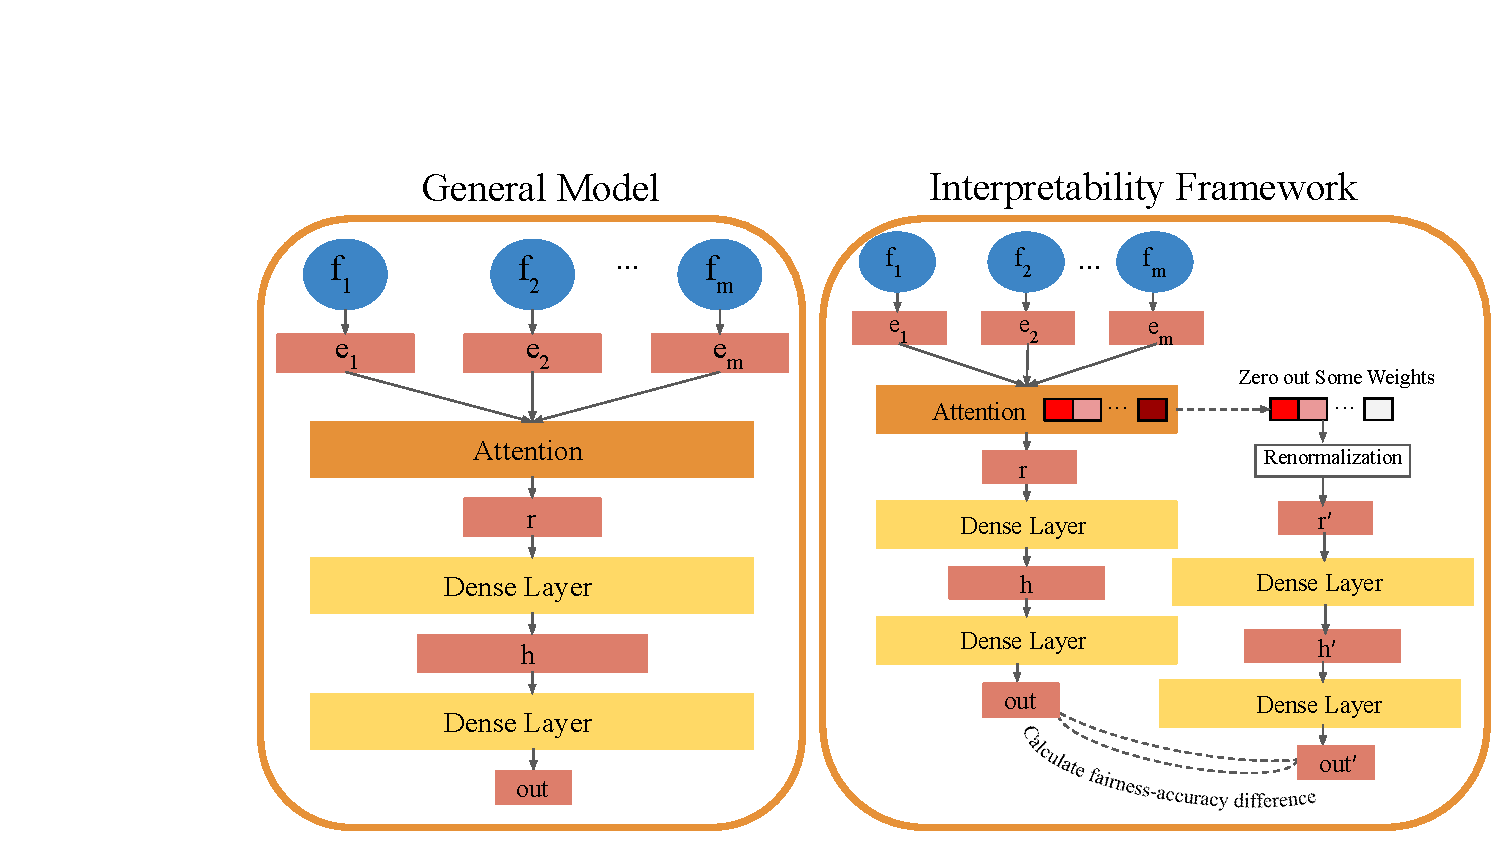
\includegraphics[width=0.96\textwidth,trim=4.2cm 0.2cm 11.7cm 2.7cm,clip=true]{images/attention_model.pdf}
%         \caption{Classification model.}
%         \label{fig:original_model}
%     \end{subfigure}
% %
%     \begin{subfigure}[b]{0.24\textwidth}
%         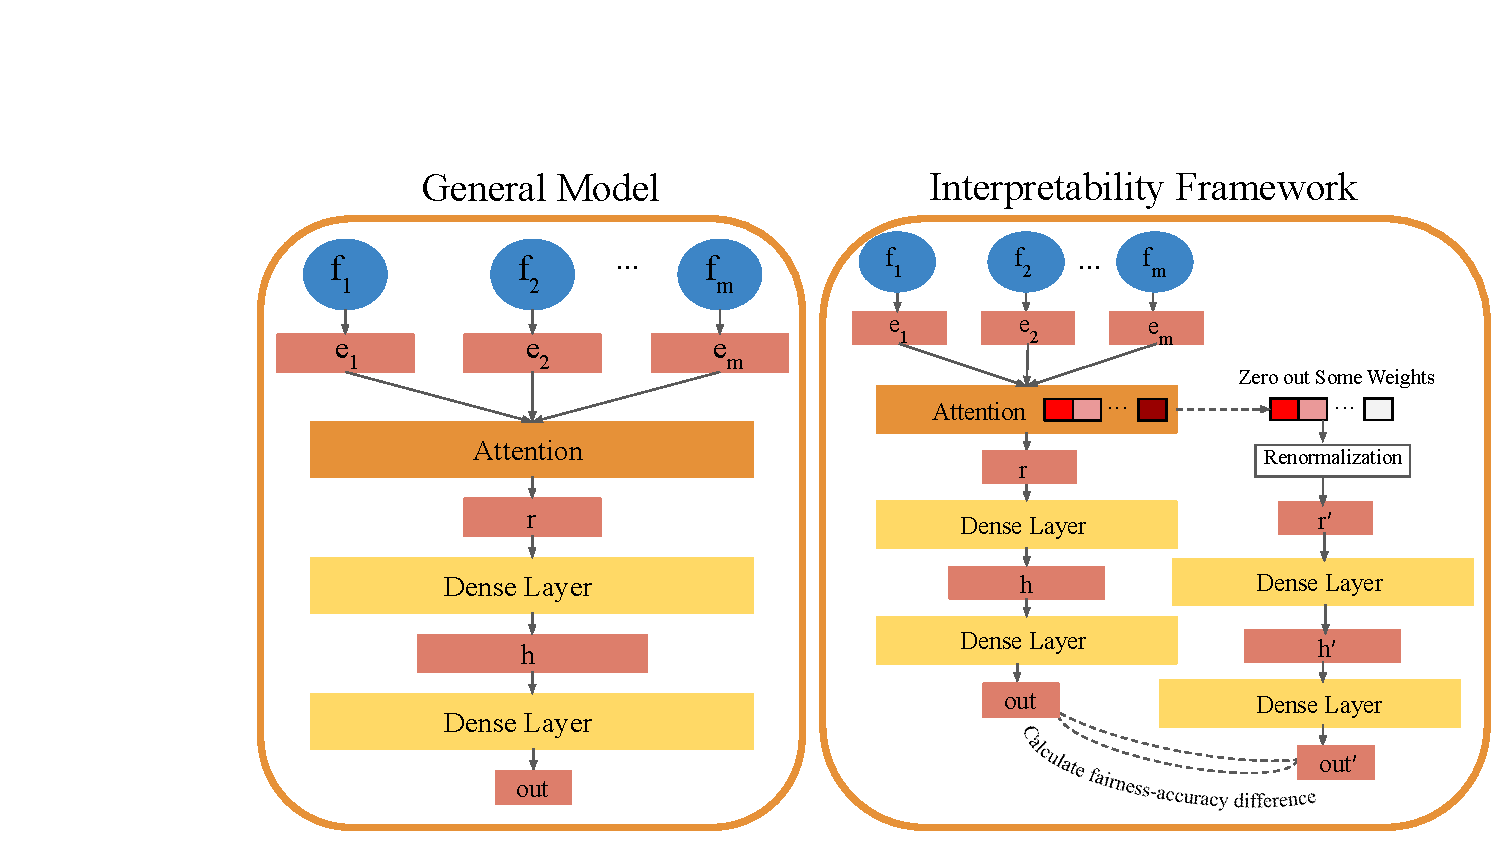
\includegraphics[width=\textwidth,trim=13.8cm 0.2cm 0.1cm 2.7cm,clip=true]{images/attention_model.pdf}
%         \caption{Interpretability framework.}
%         \label{fig:intervention_model}
%     \end{subfigure}
% %
%     \caption{(a) In general classification model, for each feature $f_i$ a vector representation $e_i$ of length $d^e$ is learned. This is passed to the attention layer which produces a $d^e$-dimensional vector representation for the whole instance which is passed to two dense layers to get the final classification output. (b) The interpretability framework has the same architecture as the general model. One outcome is obtained through the original model and another through the model that has some attention weights zeroed. The observed difference in accuracy and fairness measures will indicate the effect of the zeroed out features on accuracy and fairness.}
%     \label{fig:model}
%     %\vspace{-0.5cm}
% \end{figure}

\begin{figure}[h]
    \centering
    \begin{subfigure}[b]{0.21\textwidth}
        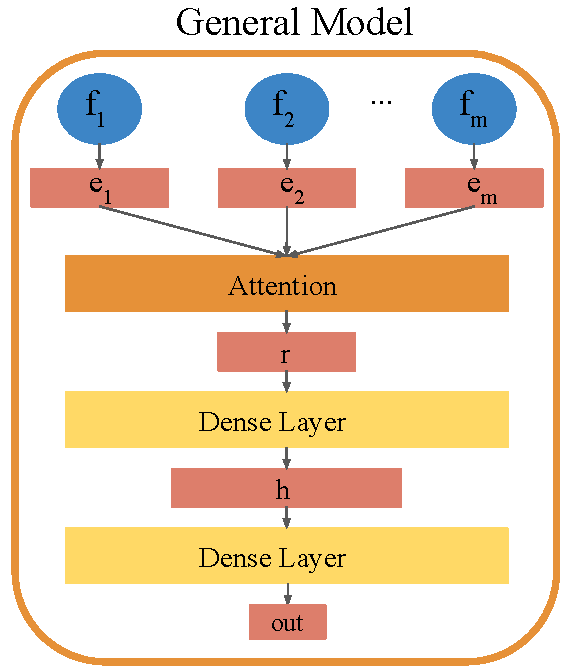
\includegraphics[width=0.96\textwidth,trim=0cm 0cm 0cm 0cm,clip=true]{images/general_model.pdf}
        \caption{Classification model.}
        \label{fig:original_model}
    \end{subfigure}
%
    \begin{subfigure}[b]{0.24\textwidth}
        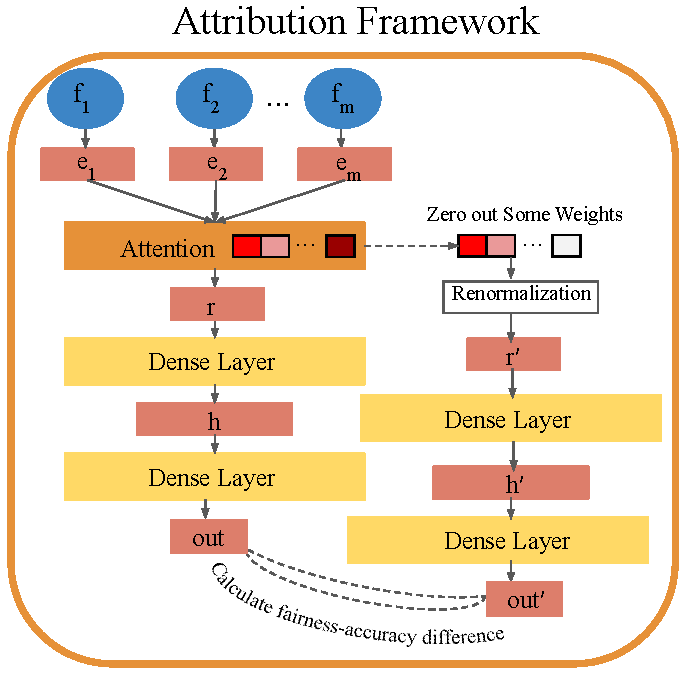
\includegraphics[width=\textwidth,trim=0cm 0cm 0cm 0cm,clip=true]{images/attr_framework.pdf}
        \caption{Attribution framework.}
        \label{fig:intervention_model}
    \end{subfigure}
%
    \caption{(a) In general classification model, for each feature $f_k$ a vector representation $e_k$ of length $d^e$ is learned. This is passed to the attention layer which produces a $d^e$-dimensional vector representation for the sample instance $i$ which is passed to two dense layers to get the final classification output. (b) The Attribution framework has the same architecture as the general model. One outcome is obtained through the original model and another through the model that has some attention weights zeroed. The observed difference in accuracy and fairness measures will indicate the effect of the zeroed out features on accuracy and fairness.}
    \label{fig:model}
    %\vspace{-0.5cm}
\end{figure}

% \begin{algorithm}[h]
% \SetAlgoLined
% Input: decay rate $d_r$ ($0 \leq d_r <1$), $n$ number of test data-points. \\
% Output: final predictions. \\
% Calculate the attention weights $\alpha$ for each $m$ existing features using the attention layer as in Eq.~\ref{eq:attention_op1}. \\
% need-decay = \{\} \\
% \For{each feature $k$}{
% Set $\alpha_o \leftarrow \alpha_k$ \\
%  Set $\alpha_k \leftarrow 0$ for all the $n$ data-point instances. \\
%     \If{$\text{SPD}(\hat {\mathbf y}_o, \mathbf {a})- \text{SPD}(\hat {\mathbf y}_z^k, \mathbf {a}) \geq 0$}{
%     need-decay = need-decay $\cup \{k\}$
%     }
%   Set $\alpha_k \leftarrow \alpha_o$ 
% }
% \For{each feature $k$}{
% \If{$k$ in need-decay}{
% Set $\alpha_k \leftarrow (d_r \times \alpha_k) $ for all the $n$ data-point instances.
% }
% }
% Use the new attention weights for all the $m$ features to obtain the final prediction outcome $\hat Y$. \\
% \Return $\hat Y$.
%  \caption{Bias Mitigation with Attention}
%  \label{mitig_alg}
% \end{algorithm}


\begin{algorithm}[h]
\SetAlgoLined
Input: decay rate $d_r$ ($0 \leq d_r <1$), $n$ test samples indexed by variable $i$. \\
Output: final predictions, unfair features. \\
Calculate the attention weights $\alpha_{ki}$ for $k^{\text{th}}$ feature in sample $i$ using the attention layer as in Eq.~\ref{eq:attention_op1}.\\
{unfair\_feature\_set} = \{\} \\
\For{each feature (index) $k$}{
% Set $\alpha_o \leftarrow \alpha_k$ \\
%  Set $\alpha_k \leftarrow 0$ for all the $n$ data-point instances. \\
    \If{$\text{SPD}(\hat {\mathbf y}_o, \mathbf {a})- \text{SPD}(\hat {\mathbf y}_z^k, \mathbf {a}) \geq 0$}{
    {unfair\_feature\_set}  = {unfair\_feature\_set}  $\cup\   \{k\}$
    }
%   Set $\alpha_k \leftarrow \alpha_o$ 
}
\For{each feature (index) $k$}{
\If{$k$ in  \text{unfair\_feature\_set}}{
Set $\alpha_{ki} \leftarrow (d_r \times \alpha_{ki})$ for all $n$ samples
}
}
Use new attention weights 
% for all the $m$ features 
to obtain the final predictions $\hat Y$. \\
\Return $\hat Y$,  {unfair\_feature\_set}
 \caption{Bias Mitigation with Attention}
 \label{mitig_alg}
\end{algorithm}

\subsection{General Model: Incorporating Attention over Inputs in Classifiers}
%\vspace{-0.2cm}
% For our general attention-based classification model, we are inspired by attention-based text classification models \cite{zhou-etal-2016-attention}. As shown on the left-hand side of Figure \ref{model}, we consider each feature value as a word in text-classification and learn a fixed-size embedding for each. We then pass these vectors $E= [e_1,e_2,...,e_n]$ to the attention layer to learn the attention weights associated to each feature, and get a representation for the instance as a whole \cite{zhou-etal-2016-attention}. Where $e_i$ is the embedding learned for the i-th feature value, $w$ is a learnable parameter, and $r$ is the representation learned for the instance that is passed to the dense layers for classification. In addition, $E \in \mathbb{R}^{d^e \times n}$ and $w$ (similar to $r$) has the same dimension as each $e_i$ ($d^e$) from which $\alpha$ attention weights will be calculated for each feature.

% The attention is over the $m$ input features. 
% For a sample indexed by $i$, 
% Umang: it is better not to introduce i, as we don't really need it here and it will complicate other notation. Example e_k will then have to e_{ki} and so on.
We consider each feature value as an individual entity (like the words are considered in text-classification) and learn a fixed-size embedding $\{e_k\}_{k=1}^m,\ e_k \in \mathbb{R}^{d^e}$ for each feature, $\{f_k\}_{k=1}^m$. These vectors are passed to the attention layer. The Computation of  attention weights and the final representation for a sample is described in Eq.~\ref{eq:attention_op1}.  $E = [e_1 \ldots e_m], \ E \in \mathbb R ^{d^e\times m}  $ is the concatenation of all the embeddings, $w \in  \mathbb{R}^{d^e} $ is a learnable parameter, $r  \in \mathbb{R}^{d^e}$ denotes the overall sample representation, and  $\alpha \in \mathbb{R}^{m}$ denotes the attention weights.
% \textcolor{red}{I put these equations in one line, but i think separating them will make it more clear. Please let me know. Umang: It looks good to me, may be we can use `,' or `;' to separate them if that looks good. Otherwise no comments }
% 
% \begin{align}
% H       & = \tanh(E)  \label{eq:attention_op1}\\
% \alpha  & = \text{softmax}(w^TH) \label{eq:attention_op2}\\
% r       & = \tanh(E\alpha^T) \label{eq:attention_op3}
% \end{align}
% 
\begin{align}
H        = \tanh(E)  \quad \label{eq:attention_op1}
\alpha   = \text{softmax}(w^TH) \quad
r        = \tanh(E\alpha^T)
\end{align}
% 
The resulting representation, $r$, is passed to the feed-forward layers for classification. In this work, we have used 
two feed-forward layers (See Fig.~\ref{fig:model} for overall architecture).
% The overall architecture is summarized in Fig.~\ref{fig:model}.

% Unlike text, we are not interested in learning dependencies between features in tabular data form; thus, we replace the LSTM layers with dense layers.

% Umang: Yeah! I think this would be redundant and we can add this in attribution section itself
% \subsection{Fairness Measures}
% In this work, we focus on group fairness measures, but our framework is applicable to other fairness measures as well. We specifically focus on statistical parity difference, equalized opportunity nad equalized odds \todo{(add citations)} and they are defined as below.

% \begin{definition}{\textbf{Statistical Parity:}}\label{def:parity}~\cite{Dwork2011}
%     It is the absolute difference between the selection rates of two groups. Mathematically,
%     \[\DP(\mathcal A, \mbc) = |P(\hat \mby = 1|\mbc=1) - P(\hat \mby=1|\mbc=0)|\]
%     where $\hat \mby$ denotes decisions produced by some decision algorithm $\mathcal A$. {When there are more than two groups, we define statistical parity to be the maximum parity between any two groups (as implemented in \citet{Bird2020}).}
% \end{definition}


% \subsection{Preliminary Notation}
% Assuming we have a binary classification task with binary sensitive attributes where $A=\{a_1,a_2\}$ represents the sensitive feature, then $\hat{y_o}=\{0,1\}$ will represent the binary outcome of the original model and $\hat{y_z}=\{0,1\}$ will represent the binary outcome of a model in which the attention weights corresponding to a feature is zeroed out. Then $y_o=\{0,1\}$ and $y_z=\{0,1\}$ represent the true labels.

% \subsection{Interpretability Framework}
% Having the aforementioned classification model with the attention mechanism, we now can observe the effect of some attributes on how they affect fairness of the outcomes by zeroing out or reducing their attention weights and recording the change according to different fairness notions. This framework is flexible in a sense that it can identify problematic attributes with regards to any fairness notion of choice. The framework is shown on the right-hand side of Figure \ref{model} in which first the outcome is recorded with the intact attention weights. Then attention weights corresponding to features can be zeroed out one by one and difference in fairness notions be recorded. Based on the observed differences one can conclude how the attribute contributes to fairness/unfairness.

% This framework is inspired by a similar work in NLP \cite{serrano-smith-2019-attention} which was trying to study the effect of attention weights on accuracy and their interpretability by comparing the difference in outcomes in terms of measures, such as Jensen-Shannon Divergence. Here, we are interested in studying fairness. Thus, the difference in outcome fairness can be calculated based on the fairness notion of choice as follows:


% \textbf{Statistical Parity:}
% \begin{align*}
%  |p(\hat{y_z}=+1|A=a_1)-p(\hat{y_z}=+1|A=a_2)|  -|p(\hat{y_o}=+1|A=a_1)-p(\hat{y_o}=+1|A=a_2)|
% \end{align*}

% \textbf{Equality of Opportunity:}
% \begin{align*}
%  |p(\hat{y_z}=+1|A=a_1,y_z=+1)&-p(\hat{y_z}=+1|A=a_2,y_z=+1)| \\ &-|p(\hat{y_o}=+1|A=a_1,y_o=+1)-p(\hat{y_o}=+1|A=a_2,y_o=+1)|
% \end{align*}

% \textbf{Equalized Odds:}
% \begin{align*}
% |p(\hat{y_z}=+1|A=a_1,y_z=y)&-p(\hat{y_z}=+1|A=a_2,y_z=y)| \\ &-|p(\hat{y_o}=+1|A=a_1,y_o=y)-p(\hat{y_o}=+1|A=a_2,y_o=y)| y \in \{0,+1\}
% \end{align*}

% Notice a value greater than zero will indicate that the attribute helps in mitigating unfairness and a value less than zero will indicate that the attribute contributes to unfairness. This is because $\hat{y_z}$ represents the exclusion of the feature (zeroed out attention weight for that feature) from the decision making process, and if the value is higher than zero, it means that not having this feature makes the bias higher than when we include the feature.
\subsection{Fairness Attribution with Attention Weights}
%\vspace{-0.2cm}
The aforementioned classification model with the attention mechanism combines input feature embeddings by taking a weighted combination. By manipulating the weights, we can intuitively capture the effects of specific features on the output.  To this end, we observe the effect of each attribute on the fairness of outcomes by zeroing out or reducing its attention weights and recording the change. Other works have used similar ideas to understand the effect of attention weights on accuracy and evaluate interpretability of the attention weights by comparing the difference in outcomes in terms of measures such as Jensen-Shannon Divergence~\cite{serrano-smith-2019-attention} but not for fairness. We are interested in the effect of features on fairness measures.  Thus, we measure the difference in fairness of the outcomes based on the desired fairness measure. A large change in fairness measure and a small change in performance of the model would indicate that this feature is mostly responsible for unfairness, and it can be dropped without causing large impacts on performance. The overall framework is shown in Fig.~\ref{fig:model}. First, the outcomes are recorded with the original attention weights intact (Fig.~\ref{fig:original_model}). Next, attention weights corresponding to a particular feature are zeroed out, and the difference in performance and fairness measures is recorded (Fig.~\ref{fig:intervention_model}). Based on the observed differences, one may conclude how incorporating this feature contributes to fairness/unfairness.

To measure the effect of the $k^{th}$ feature on different fairness measures, we consider the difference in the fairness of outcomes of the original model and model with $k^{th}$ feature's effect removed. For example, for statistical parity difference, we will consider $\text{SPD}(\hat {\mathbf y}_o, \mathbf {a})- \text{SPD}(\hat {\mathbf y}_z^k, \mathbf {a})$. A negative value will indicate that the $k^{th}$ feature helps mitigate unfairness, and a positive value will indicate that the $k^{th}$ feature contributes to unfairness. This is because $\hat{y}_z^k$ captures the exclusion of the $k^{th}$ feature (zeroed out attention weight for that feature) from the decision-making process. If the value is positive, it indicates that not having this feature makes the bias lower than when we include it. Notice here, we focus on global attribution, so we measure this over all the samples; however, this can also be turned into local attribution by focusing on individual sample $i$ only.
%\vspace{-0.2cm}
\subsection{Mitigating Bias by Removing Unfair Features} \label{mitig_sec}
%\vspace{-0.2cm}
As discussed in the previous section, we can identify features that contribute to unfair outcomes according to different fairness measures. A simple technique to mitigate or reduce bias is to reduce the attention weights of these features. This mitigation technique is outlined in Algorithm~\ref{mitig_alg}. In this algorithm, we first individually set attention weights for each of the features in all the samples to zero and monitor the effect on the desired fairness measure. We have demonstrated the algorithm for SPD, but other measures, such as EqOdd, EqOpp, and even accuracy can be used (in which case the ``unfair\_feature\_set'' can be re-named to feature set which harms accuracy instead of fairness). If the $k^{th}$ feature contributes to unfairness, we reduce its attention weight using decay rate value. This is because $\hat {\mathbf y}_z^k$ captures the exclusion of the $k^{th}$ feature (zeroed attention weight for that feature) compared to the original outcome $\hat {\mathbf y}_o$ for when all the feature weights are intact; otherwise, we use the original attention weight. We can also control the fairness-accuracy trade-off by putting more attention weight on features that boost accuracy while keeping the fairness of the model the same and down-weighting features that hurt accuracy, fairness, or both. 

This post-processing technique has a couple of advantages over previous works in bias mitigation or fair classification approaches. First, the post-processing approach is computationally efficient as it does not require model retraining to ensure fairness for each sensitive attribute separately. Instead, the model is trained once by incorporating all the attributes, and then one manipulates attention weights during test time according to particular  needs and use-cases. Second, the proposed mitigation method provides an explanation and can control the fairness-accuracy trade-off. 
This is because manipulating the attention weights reveals which features are important for getting the desired outcome, and by how much.
% This is because manipulating the attention weights reveals what features were manipulated to get the desired outcome, and by how much. 
This provides an explanation for the outcome and also a mechanism to control the fairness-accuracy trade-off by the amount of the manipulation.

%We demonstrate competitive trade-off curves compared to several recent approaches.

%3. The model can be trained once and given as a black-box model to the practitioner. The practitioner can then control the importance of each attribute during test time to satisfy what they care about the most (accuracy, or fairness, or both).


% Using the interpretability framework explained in the previous section and identifying the problematic features, one can design a post-processing bias mitigation technique by manipulating the attention weights of the problematic features. Using the interpretability framework, one can also control the fairness-accuracy trade-off by putting more attention weight to features that are boosting the accuracy while keeping the fairness of the model the same and down-weighting features that are hurting the accuracy, fairness, or both.

% This post-processing technique has couple of advantages over previous work in bias mitigation or fair classification models: 1. This post-processing approach can save time and energy since it is not required to retrain the model to ensure fairness for each sensitive attribute separately. The model needs to be trained once by incorporating all the attributes and only during test time the attention weights can be manipulated according to the needs and use-cases of the user. 2. It provides explanation and can control the fairness-accuracy trade-off. 3. The model can be trained once and given as a black-box model to the practitioner. The practitioner can then control the importance of each attribute during test time to satisfy what they care about the most (accuracy, or fairness, or both).


